Until now, we have so far taken a computational task as a function (\textit{that takes input a string and returns another string}) or a language (\textit{that 
takes in input a string and returns a boolean value}). Below, we have a picture about the two representations: the left-most is a function, while the right-most
is a language. \vspace{3.5pt}
\begin{center}
    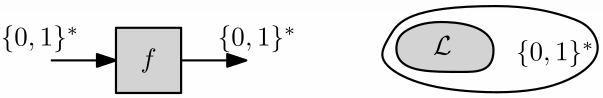
\includegraphics[width = 0.6\textwidth]{img/img5.png}
\end{center} \vspace{3.5pt}
However, can \textbf{learning problems} be seen as \textbf{computational problems}? The answer is positive: any learning algorithm $A$ can be seen as an algorithm
computing a function $f_A$ whose input is a finite sequence of \textbf{labelled data} and whose output can be seen as a \textbf{classifier}. \vspace{3.5pt}
\begin{center}
    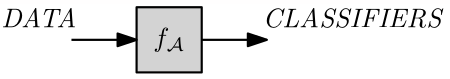
\includegraphics[width = 0.5\textwidth]{img/img6.png}
\end{center} \vspace{3.5pt}
Conversely of what we did in \textbf{computation theory}, the output is not anymore a string or a boolean value but instead a \textbf{classifier}, in other words 
another function. This new type of output, namely a function, is a classifier able to categorize new data similar to the input labelled data. \vspace{7pt}

The previous observatons lead us to the following questions:
\begin{enumerate}
    \item Could data and classifiers be encoded as strings, such that $f_A$ becomes a function of the kind we already know?
    \item How could we formalize the fact that $A$ correctly solves a given learning task?
\end{enumerate} \vspace{7pt}

More in details, the discussion done until now can be figured as in the image below. \vspace{3.5pt}
\begin{center}
    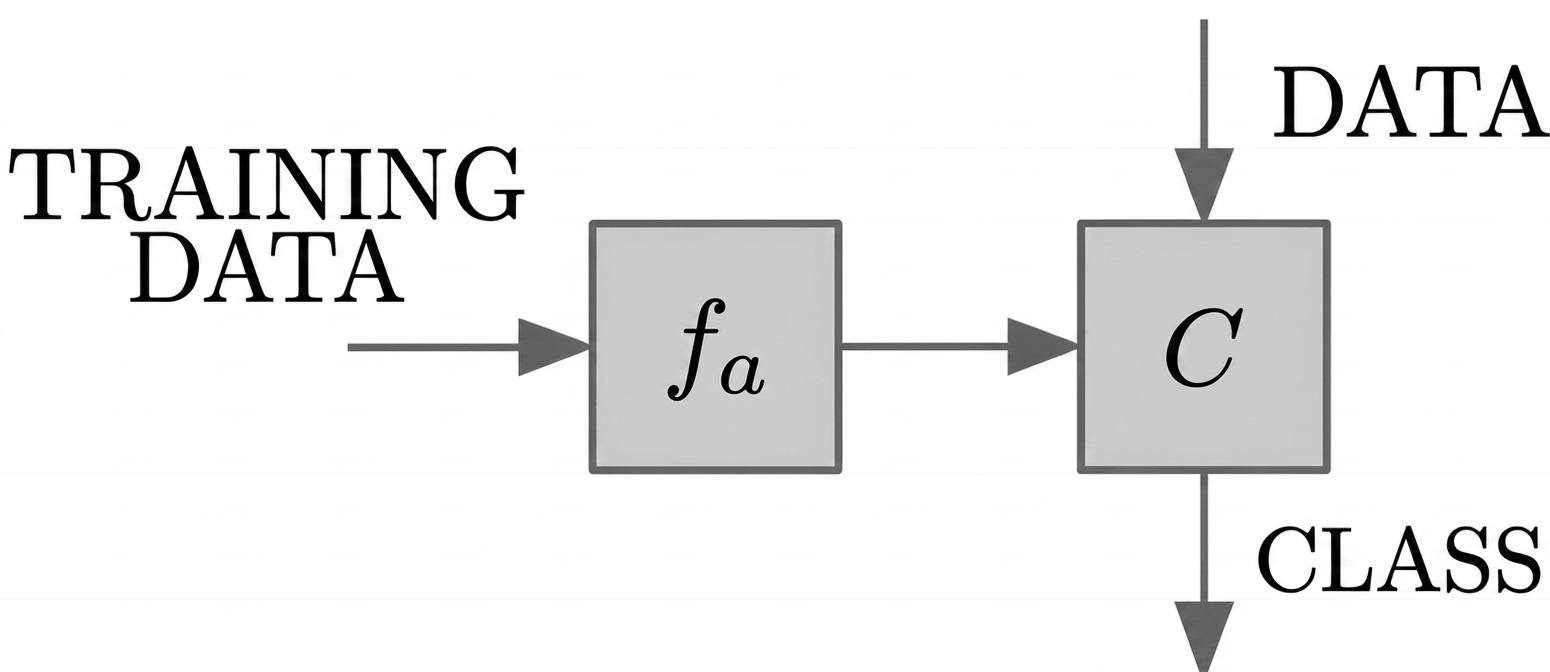
\includegraphics[width = 0.5\textwidth]{img/img7.png}
\end{center} \vspace{3.5pt}
It's a kind of pipeline, divided into the following steps:
\begin{enumerate}
    \item \textbf{Training data}, we get training data in order to \textbf{train} our model, in particular to recognize interesting patterns over the labelled data.
    \item $\boldsymbol{f_A}$, computing the function $f_A$ we learn the relationship between data and labels.
    \item $\boldsymbol{C}$, output after the computation of the function $f_A$, which is itself a function, in particular a classifier.
    \item \textbf{Data}, data coming in the classifier $C$ are \textbf{not labelled data}.
    \item \textbf{Class}, the real task of the classifier $C$ is to find out an appropriate label of any \textbf{unlabelled data} given in input to it.
\end{enumerate}